\section{Method}
\label{sec:method}

We introduce \nameMethod, a method that takes a source video $\sourcevideo \in \videospace$ as input and synthesizes a target video $\targetvideo \in \videospace$, following an input camera trajectory $\camera_{\trg}\in \mathbb{R}^{\numf \times 3 \times 4}$ and temporal control signal $\animatime_{\trg} \in \mathbb{R}^{\numf}$.
Here, $\numf$ denotes the number of frames, $\numchannel$ the number of color channels, 
and $\height$ and $\width$ are the frame height and width, respectively. 
Each $\camera_{\trg}^{f} \in \mathbb{R}^{3 \times 4}$ represents the camera extrinsic 
parameters (rotation and translation) at frame $f$, with respect to the 1\textsuperscript{st} frame of  $\sourcevideo$.
The target video $\targetvideo$ preserves the scene’s underlying dynamics, geometry, and appearance in $\sourcevideo$, while adhering to the camera motion and temporal progression specified by $\camera_{\trg}$ and $\animatime_{\trg}$.
A key feature of our method is the disentanglement of spatial and temporal factors in the generative process, enabling effects such as bullet-time and retimed playback from novel viewpoints (see \cref{fig:teaser}).



\subsection{Preliminaries}
Our framework builds upon recent advances in large-scale text-to-video diffusion models and camera-conditioned video generation. 
We adopt a latent video diffusion backbone similar to modern text-to-video foundation models \cite{wan2025}, consisting of a 3D Variational Auto-Encoder (VAE) for latent compression and a Transformer-based denoising model (DiT) operating over multi-modal tokens. 

Additionally, our design draws inspiration from \recammaster~\cite{Bai2025}, which introduces explicit camera conditioning for video synthesis. 
Given an input camera trajectory $\camera \in \mathbb{R}^{\numf \times 3 \times 4}$, 
spatial conditioning is achieved by first projecting the camera sequence to the space of video tokens and adding it to the features:
\begin{equation}
x' = x + \camencoder\left(\camera\right),
\label{eq:camera-condition}
\end{equation}
where $x$ is the output of the patchifying module and $x'$ is the input to self-attention layers. 
The camera encoder $\camencoder$ maps each flattened $3 \times 4$ camera matrix (12-dimensional) into the target feature space, while also transforming the temporal dimension from $\numf$ to $\numflt$.

\subsection{Disentangling Space and Time}
We achieve spatial and temporal disentanglement through a two-fold approach: a dedicated time representation and specialized datasets.

\subsubsection{Time representation}
\label{sec:time_embedding}
Recent video diffusion models include position embeddings for latent frame index $f'$, such as RoPE($f'$). 
However, we found using RoPE($f'$) for temporal control to be ineffective, as it interferes with camera signals: RoPE($f'$) often constrains both temporal and camera motion simultaneously.
To address space and time disentanglement, we introduce a dedicated time control parameter $\animatime \in \mathbb{R}^F$.
By manipulating $\animatime_\trg$, we can control the temporal progression of the synthesized video $\targetvideo$. For example, setting $\animatime_\trg$ to a constant locks $\targetvideo$ to a specific timestamp in $\sourcevideo$, while reversing the frame indices produces a playback of $\sourcevideo$ in reverse.
\begin{figure}[t]
    \centering
    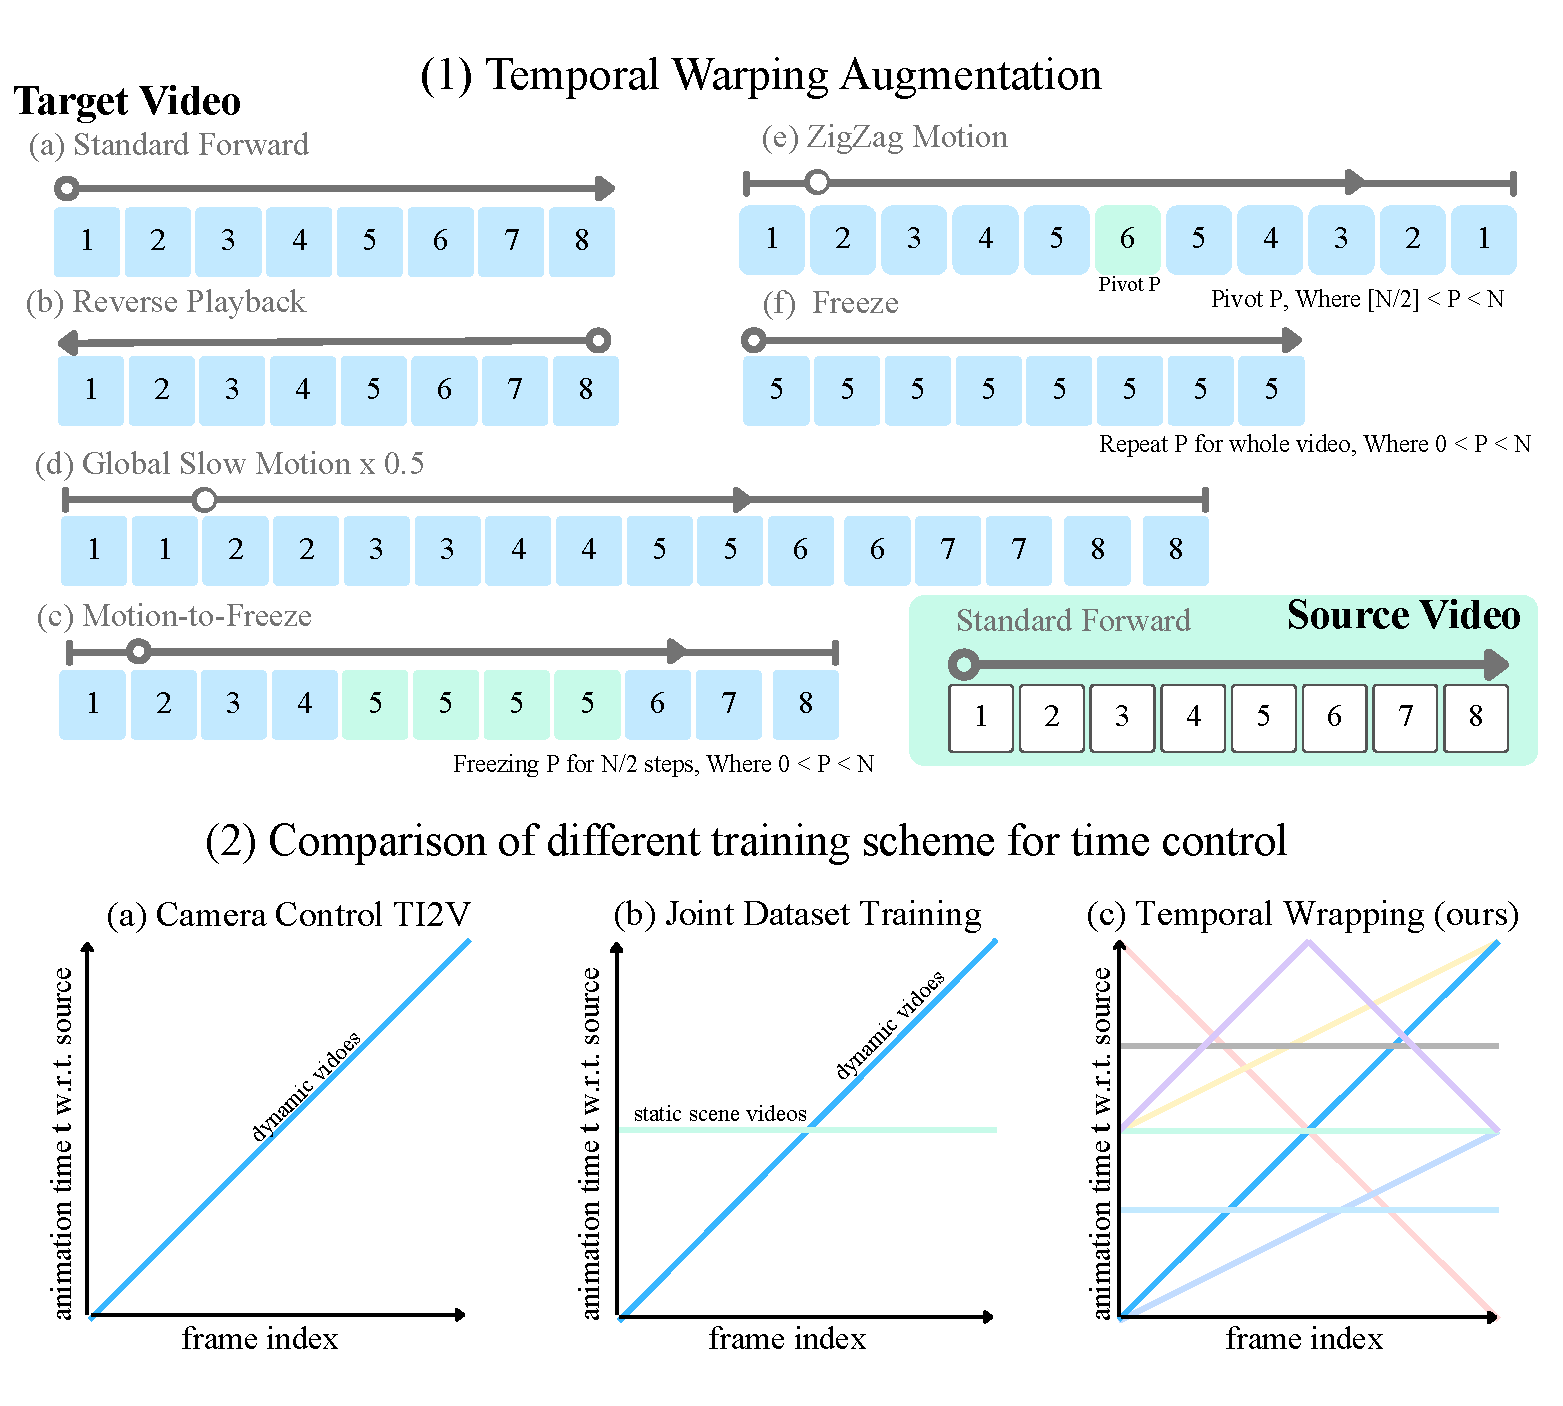
\includegraphics[width=\linewidth]{figures/src_files/TWA.pdf}
    \vspace{-0.5cm}
    \caption{
        \textbf{Temporal Wrapping for Spatiotemporal Disentanglement.}
        (Top) For multi-view dynamic scene datasets \cite{Bai2025}, a set of temporal warping operations (e.g.\, reverse playback, zigzag motion, slow motion, and freeze) are applied to the target video, with the source video kept as the standard forward reference, providing explicit supervision for temporal control  .
        (Bottom) Compared with existing camera-control \cite{vanhoorick2024gcd, Bai2025} and joint-dataset training strategies \cite{Wu2024, watson2025controllingspacetimediffusion}, which rely on monotonic time progression and static-scene videos to demonstrate temporal differences, Temporal Wrapping provide much more diverse and explicit signals of temporal variation, leading to disentanglement of space and time.
    }
    \label{fig:temporal_wrapping}
    \vspace{-0.3cm}
\end{figure}


(Top) For multi-view dynamic scene datasets, a set of temporal warping operations, including reverse, playback, zigzag motion, slow motion, and freeze are apppplied with teh source video as standford. This gives explicit supervision for temporal control, without constructing additional temporally varied training data.

(Bottom) Existing camera-control and joint dataset training rely on monotonic time progression and static scene videos, making it difficult for models to understand temporal variation. The introduced temporal mappings from multi-view video data, which provide diverse and clear signal on tempral variation, and directly lead to disentanglement of space and time.

\myparagraph{Time Embedding.}
To inject temporal control into the diffusion model, we analyze several approaches. 
First, we can encode time similar to a frame index using RoPE embedding. 
However, we find it less suitable for time control (\todo{visual evaluations are provided in \suppmat}).
Instead, we adopt sinusoidal time embeddings applied at the latent frame $f'$ level, which provide a stable and continuous representation of each frame’s temporal position and offer a favorable trade-off between precision and stability. 
We further observe that each latent frame corresponds to a continuous temporal chunk, and propose using embeddings of original frame indices $f$ to support finer granularity of time control. 
To accomplish this, we introduce a time encoding approach $\animaencoder(\animatime)$, where $\animatime \in \mathbb{R}^F$. 
We first compute the sinusoidal time embeddings to represent the temporal sequence, $\mathbf{e}_\src = \mathrm{SinPE}\!\left(\animatime_\src\right)$, $\mathbf{e}_\trg = \mathrm{SinPE}\!\left(\animatime_\trg\right)$, where  $\animatime_\src, \animatime_\trg \in \mathbb{R}^F$.
Next, we apply two 1D convolution layers to progressively project these embeddings into the latent frame space, $\widetilde{\mathbf{e}} = \mathrm{Conv1D_2}(\mathrm{Conv1D_1}(\mathbf{e}))$.
Finally, we add these time features to the camera features and video tokens embeddings, updating \cref{eq:camera-condition} as follows:
\begin{equation}
    x' = x + \camencoder\left(\camera\right) + \animaencoder\left(\animatime\right).
    \label{eq:cam-and-ani-condition}
\end{equation}

In \cref{sec:time_embedding_ablation}, we compare our approach with alternative conditioning strategies, such as using sinusoidal embeddings where $\animatime_\src,\animatime_\trg$ are directly defined in $\mathbb{R}^{F'}$, and employing an MLP instead of a 1D convolution for compression. We demonstrate both qualitatively and quantitatively the advantages of our proposed method.



\subsubsection{Datasets}
\label{sec:datasets}
To enable temporal manipulation in our approach, we require paired training data that includes examples of time remapping. 
Achieving spatial-temporal disentanglement further requires data containing examples of both camera and temporal controls. 
To the best of our knowledge, no publicly available datasets satisfy these requirements.
Only a few prior works, such as \fourdim \cite{watson2025controllingspacetimediffusion} and \catfourd \cite{Wu2024}, have attempted to address spatial-temporal disentanglement. 
A common strategy is to jointly train on static-scene datasets and multi-view video datasets \cite{zhou2018stereo,ling2024dl3dv}. 
The limited control variability in these datasets leads to confusion between temporal evolution and spatial movement, resulting in entangled or unstable behaviors \cite{watson2025controllingspacetimediffusion,Wu2024}. 
We address this limitation by augmenting existing multi-view video data with temporal warping and by proposing a new synthetic dataset.


\myparagraph{Temporal Warping Augmentation.}
We introduce simple augmentations that add controllable temporal variations to multi-view video datasets.
During training, given a source video $\sourcevideo = \{I_\src^f\}_{f=1}^{F}$ and a target video $\targetvideo = \{I_\trg^f\}_{f=1}^{F}$, we apply a temporal warping function $\tau: [1, \numf] \rightarrow [1, \numf]$ to the target sequence, producing a warped video $V_\trg' = \{I_\trg^{\tau(f)}\}_{f=1}^{F}$. 
The source animation timestamps are uniformly sampled, $\animatime_\src = 1:F$. 
Warped timestamps, $\animatime_\trg = \tau(\animatime_\src)$, introduce non-linear temporal effects (see \cref{fig:temporal_wrapping} top b–e): (i) reversal, (ii) acceleration, (iii) freezing, (iv) segmental slow motion, and (v) zigzag motion, in which the animation repeatedly reverses direction.
After these augmentations, the paired video sequences $(V_\src, V_\trg')$ differ in both camera trajectories and temporal dynamics, providing the model with a clear signal for learning disentangled spatiotemporal representations.




\begin{table}[!t]
  \centering
  \definecolor{Gray}{gray}{0.9}
  \caption{
\textbf{Comparison of existing multi-view datasets for camera and temporal control against Cam$\times$Time.} Cam$\times$Time provides full-grid rendering (Figure~\ref{fig:dataset_blender}), enabling target videos to sample arbitrary temporal variations over the full range from 0 to 120.
  }
  \vspace{-0.2cm}
  \label{tab:dataset-comparison}
  \begin{adjustbox}{max width=\columnwidth}
  \begin{tabular}{l|c|c|c|c}
    \toprule
     Dataset & Dynamic scenes & Src. Time: $t_{\text{src}}$ & Tgt. Time: $t_{\text{trg}}$ & Camera \\
    \midrule
    \midrule
    RE10k \cite{zhou2018stereo} & \redxmark & 1 & 1 & Moving \\
    DL3DV10k \cite{ling2024dl3dv} & \redxmark & 1 & 1 & Moving \\
    MannequinChallenge \cite{rockwell2025dynpose} & \redxmark & 1 & 1 & Moving \\
    Kubric-4D \cite{vanhoorick2024gcd} & \greencmark & 1:60 & 1:60 & Moving \\
    ReCamMaster \cite{Bai2025} & \greencmark & 1:80 & 1:80 & Moving \\
    SynCamMaster \cite{bai2024syncammaster} & \greencmark & 1:80 & 1:80 & Fixed \\
    \midrule
        \rowcolor{Gray}
    \textbf{Cam$\times$Time (ours)} & \greencmark & 1:120 & $\{1, 2, \dots, 120\}^{120}$ & Moving \\
    \bottomrule
  \end{tabular}
  \end{adjustbox}
  \vspace{-3.5mm}
\end{table}

\myparagraph{Synthetic \nameDataset Dataset for Precise Spatiotemporal Control.}
While our temporal warping augmentations encourage strong disentanglement between spatial and temporal factors, achieving fine-grained and continuous control --- that is, smooth and precise adjustment of temporal dynamics --- benefits from a dataset that systematically covers both dimensions.
To this end, we construct \textit{\nameDataset}, a new synthetic spatiotemporal dataset rendered in Blender. 
Given a camera trajectory and an animated subject, \nameDataset exhaustively samples the camera–time grid, capturing each dynamic scene across diverse combinations of camera viewpoints and temporal states $\left(\camera, \animatime\right)$, as illustrated in \cref{fig:dataset_blender}.
The source video is obtained by sampling the diagonal frames of the dense grid (\cref{fig:dataset_blender} (bottom)), while the target videos are obtained by more free-form sampling of continuous sequences. 
We compare \nameDataset against existing datasets in \cref{tab:dataset-comparison}. 
While \cite{zhou2018stereo,ling2024dl3dv,rockwell2025dynpose} are real videos with complex camera path annotations, they either do not provide time-synchronized video pairs \cite{rockwell2025dynpose} or only provide pairs of static scenes \cite{ling2024dl3dv,zhou2018stereo}.
Synthetic multi-view video datasets \cite{Bai2025,bai2024syncammaster,vanhoorick2024gcd} provide pairs of dynamic videos but do not allow training for time control. 
In contrast, \nameDataset enables fine-grained manipulation of both camera motion and temporal dynamics, enabling bullet-time effects, motion stabilization, and flexible combinations of the controls.
We designate part of \nameDataset as a test set, aiming for it to serve as a benchmark for controllable video generation.
We will release it to support future research on fine-grained spatiotemporal modeling.






\begin{figure}[t]
    \centering
    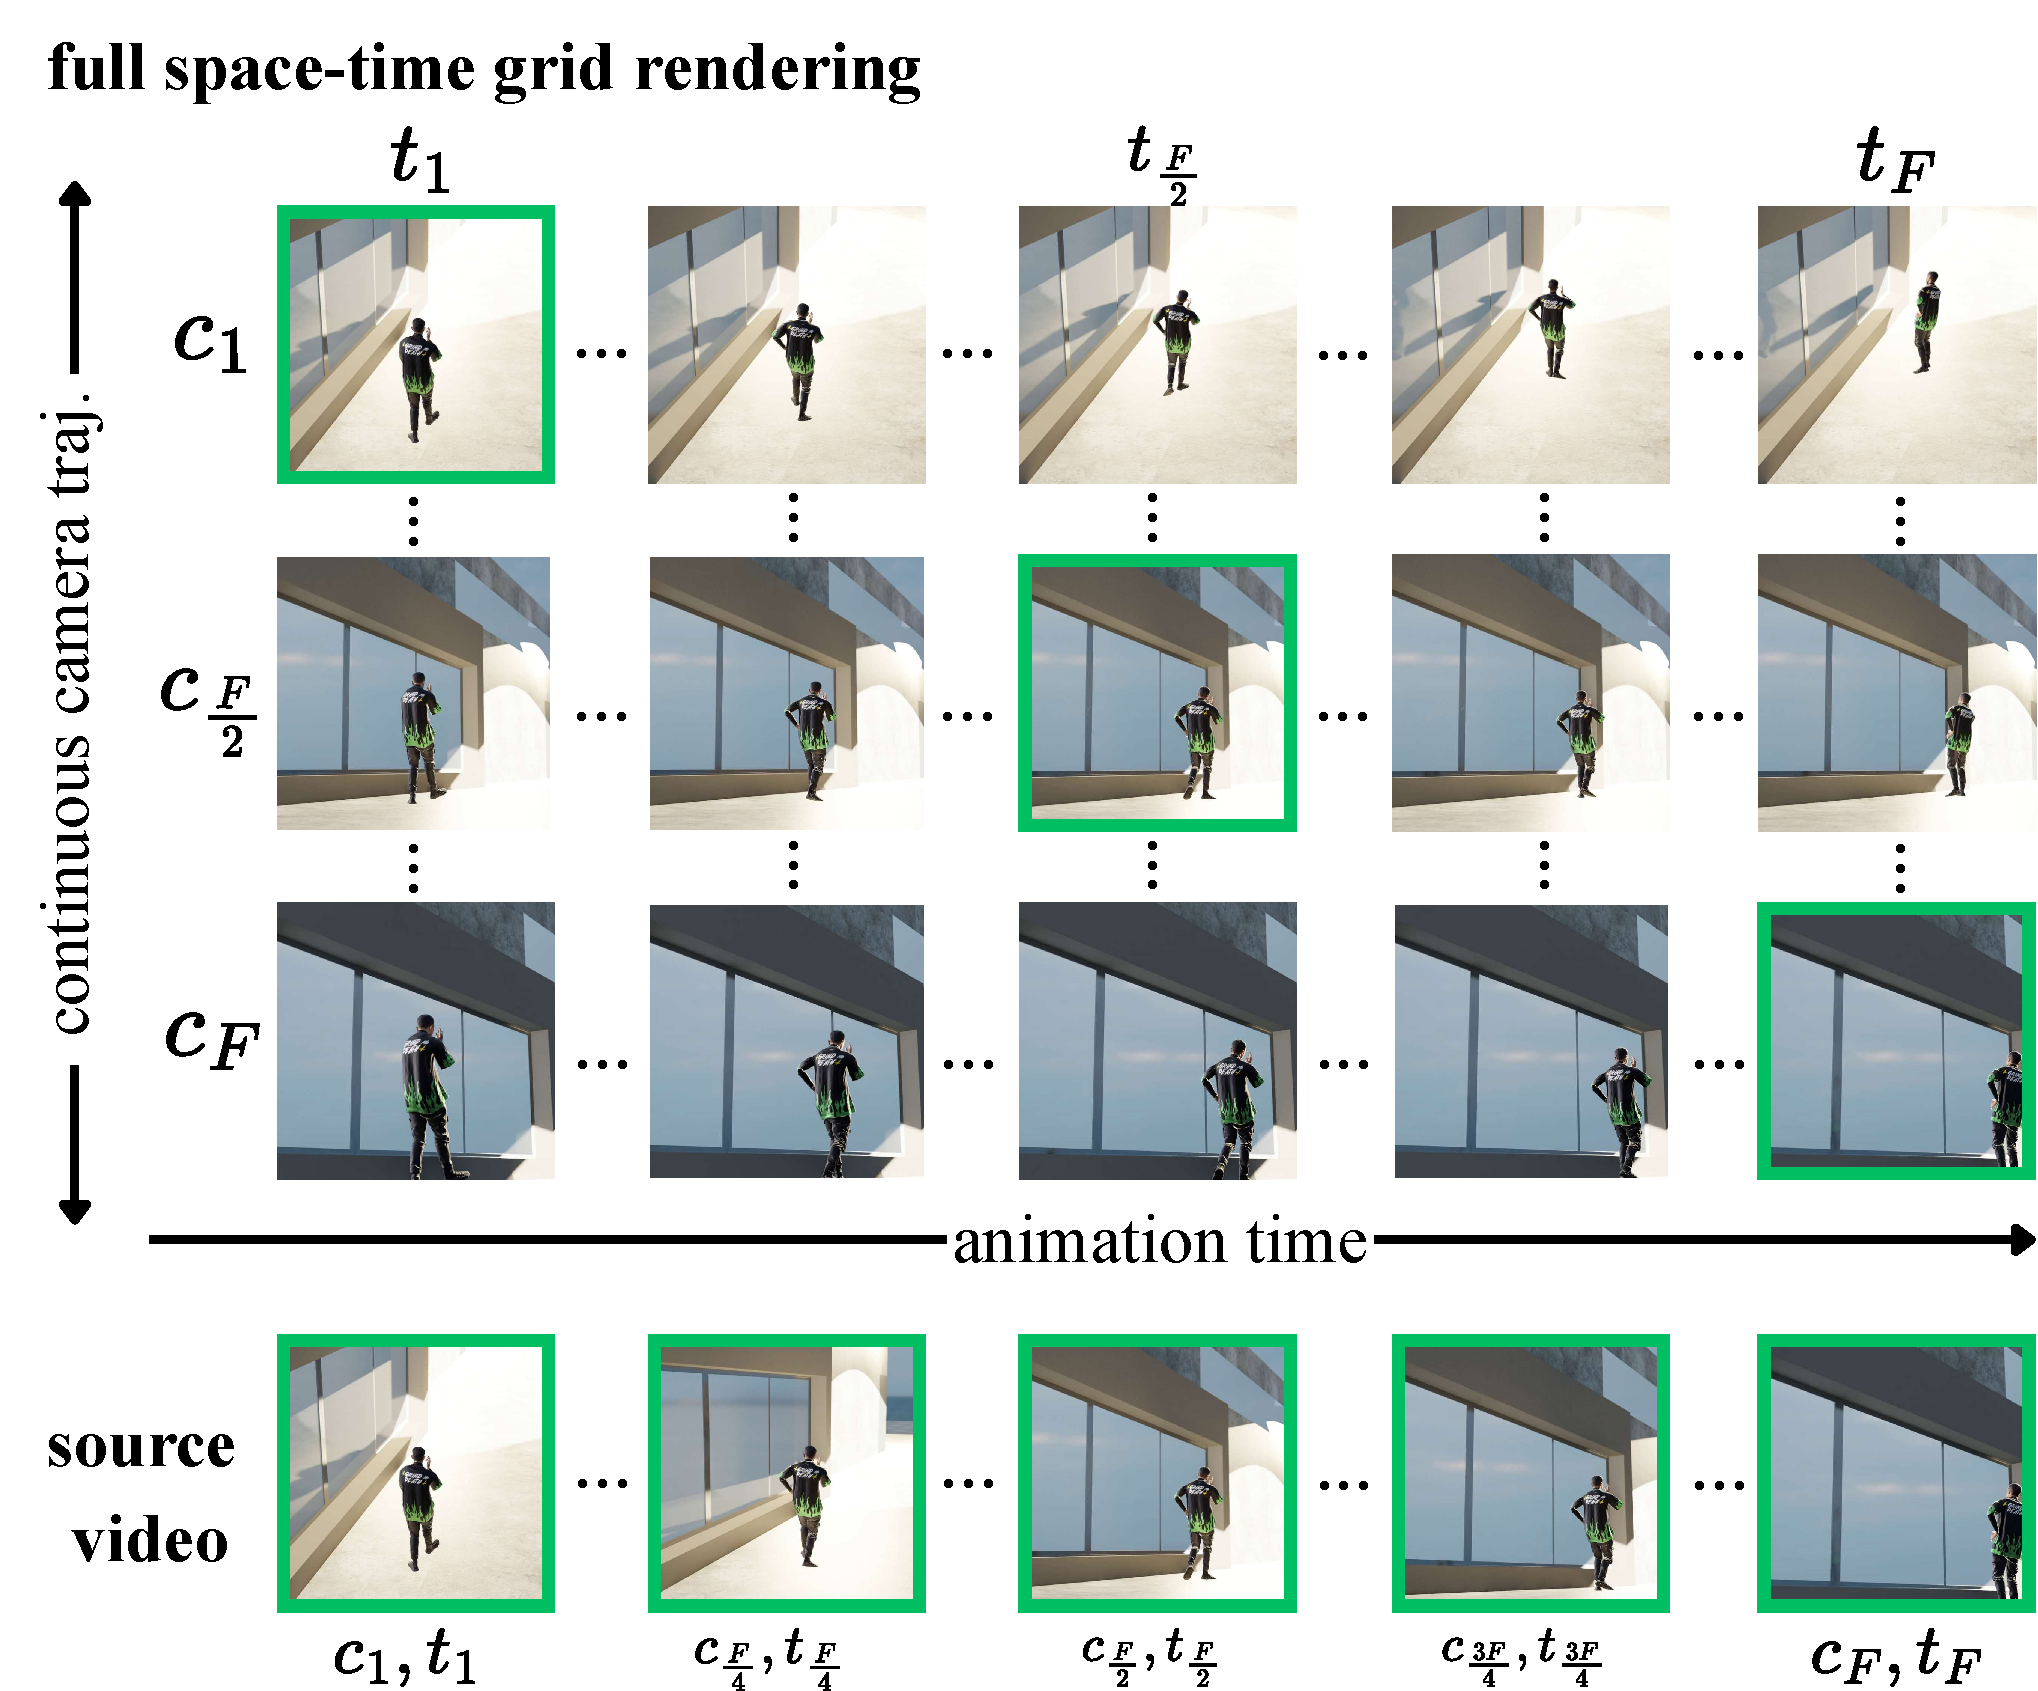
\includegraphics[width=\columnwidth,trim={0 0 0 3mm},clip]{figures/src_files/dataset.pdf}
    \caption{
    \textbf{\textit{\nameDataset} dataset visualization}. (Top) A space-time grid defined by a camera trajectory $\camera=[c_1,...,c_F]$ and animation status $\animatime=[t_1,...,t_F]$. \nameDataset renders images for all $(c,t)$ pairs, covering the full grid for learning disentangled spatial and temporal control. Any two sampled  sequences of $\numf$ frames from the grid can form a source-target pair. (Bottom) One typical choice of source videos is taking the diagonal cells in     green. }
    \label{fig:dataset_blender}
    \vspace{-0.3cm}
\end{figure}


\begin{table*}[t]
    \centering
    \caption{
        Quantitative comparison across temporal controls 
        (\textit{Direction (forward, backward motion)}, \textit{Speed (slow modes)}, \textit{Bullet Time}).
        We report PSNR$\uparrow$, SSIM$\uparrow$, and LPIPS$\downarrow$.
        Best results are in \textbf{bold}. SpaceTimeMethod showcase best performance for temporal control overall.
    }
    \vspace{-0.2cm}
    \label{tab:temporal_eval}
    \small
    \setlength\tabcolsep{3.6pt}  %
    \begin{tabular}{l|ccc|c|ccc|c|ccc|c}
        \toprule
        \multirow{2}{*}{\textbf{Method}} &
        \multicolumn{4}{c|}{\textbf{PSNR$\uparrow$}} &
        \multicolumn{4}{c|}{\textbf{SSIM$\uparrow$}} &
        \multicolumn{4}{c}{\textbf{LPIPS$\downarrow$}} \\
        \cmidrule(lr){2-5} \cmidrule(lr){6-9} \cmidrule(lr){10-13}
         & Dir. & Speed & Bullet & Avg
         & Dir. & Speed & Bullet & Avg
         & Dir. & Speed & Bullet & Avg \\
        \midrule

        ReCamM+preshuffled$^\dagger$
        & 17.13 & 14.84 & 14.61 & 15.52
        & 0.6623 & 0.6050 & 0.5965 & 0.6213
        & 0.3930 & 0.4793 & 0.4863 & 0.4529 \\

        ReCamM+jointdata
        & 18.32 & 17.57 & 17.69 & 17.86
        & 0.7322 & 0.7220 & 0.7209 & 0.7250
        & 0.2972 & 0.3158 & 0.3089 & 0.3073 \\

        \textbf{\nameMethod (Ours)}
        & \textbf{21.75} & \textbf{20.87} & \textbf{20.85} & \textbf{21.16}
        & \textbf{0.7725} & \textbf{0.7645} & \textbf{0.7653} & \textbf{0.7674}
        & \textbf{0.1697} & \textbf{0.1917} & \textbf{0.1677} & \textbf{0.1764} \\
        \bottomrule
    \end{tabular}

    {\footnotesize
    $^\dagger$\,Uses simple frame-rearrangement operators 
    (reversal, repetition, freezing) applied prior to inference to emulate 
    temporal manipulation.}
    \vspace{-0.3cm}
\end{table*}


\subsection{Precise Camera Conditioning}
\label{sec:src_cam}
We aim for full camera trajectory control in the target video.
In contrast, the previous novel-view synthesis approach \cite{Bai2025} assumes that the first frame is identical in source and target videos and that the target camera trajectory is defined relative to it. 
This stems from the two limitations. 
First, the existing approach ignores the source video trajectory, yielding suboptimal source features computed using the target trajectory for consistency:
\[
x_\src' = x_\src + \camencoder\left(\camera_\trg\right), \quad x_\trg' = x_\trg+ \camencoder\left(\camera_\trg\right).
\]
Second, it is trained on datasets where the first frame is always identical across the source and target videos. 
This latter limitation is addressed in our training datasets design.

To overcome the former, we devise a \textit{source-aware camera conditioning}. 
We estimate camera poses for both the source and target videos using a pretrained pose estimator, and inject them jointly into the diffusion model to provide explicit geometric context. Eq.~\ref{eq:cam-and-ani-condition} is therefore extended into:
\begin{align}
&x_\src' = x_\src + \camencoder\left(\camera_\src\right) + \animaencoder\left(\animatime_\src\right), \label{eq-srccam} \\
&x_\trg' = x_\trg + \camencoder\left(\camera_\trg\right) + \animaencoder\left(\animatime_\trg\right), \nonumber \\
&x' = [x_\trg', x_\src']_{\text{frame-dim}}, \nonumber
\end{align}
where $x'$ denotes the input of the \dit model, which is the concatenation of target and source tokens along the frame dimension. This formulation provides the model with both source and target camera context, enabling spatially consistent generation and precise control over camera trajectories.







\subsection{Support for Longer Video Segments}
\label{sec:LongerVideoSegements}
Finally, to showcase the full potential of our camera and temporal control, we adopt a simple autoregressive video generation strategy, generating each new segment $V_{\trg}$ conditioned on the previously generated segment $V_{\prv}$ and a source video $V_{\src}$ to produce longer videos. 

To enable this capability during inference, we need to extend our training scenario to support conditioning on two videos, where one serves as $V_{\src}$ and the other as $V_{\prv}$.
The source video $V_{\src}$ is taken directly from the multi-view datasets or from our synthetic dataset, as was described previously. 
$V_{\prv}$ is constructed in a similar way to $V_{\trg}$ --- either using temporal warping augmentations or by sampling from the dense space-time grid of our synthetic dataset. 
When temporal warping is applied, $V_{\prv}$ and $V_{\trg}$ may originate from the same or different multi-view sequences representing the same time interval. 
To maintain full flexibility of control, we do not enforce any other explicit correlations between $V_{\prv}$ and $V_{\trg}$, apart from specifying camera parameters relative to the selected source video frame.

Note that not constraining the source and target videos to share the same first frame (as discussed in \cref{sec:src_cam}) is crucial for achieving flexible camera control in longer sequences.
For instance, this design enables extended bullet-time effects: we can first generate a rotation around a selected point up to $45^\circ$ ($V_{\trg,1}$), and then continue from $45^\circ$ to $90^\circ$ ($V_{\trg,2}$).
Conditioning on two consecutive source segments allows the model to leverage information from newly generated viewpoints.
In the bullet-time example, conditioning on the previously generated video enables the model to incorporate information from all newly synthesized viewpoints, rather than relying solely on the viewpoint of the corresponding moment in the source video.




